\section{The Slab Model Based EDA}  \label{sec:nslab} 
A major assumption of our fiducial DEM is that we sample the amplitude of
attenuation from the slab model. The slab model makes the simplifying assumption 
that dust in galaxies are in a slab-like geometry and illuminated by the
stellar radiation source~\citep{somerville1999}. Then, for a given $\tau_V$,
the attenuation depends solely on the orientation of the galaxy. This
simplification, ignores any complexities in the star-to-dust geometry that
impact the shape of the attenuation curve (\todo{Witt Gordon 1996, 2000, Seon
Drain 2016}). 

Besides its simplifications, the slab model predicts $A_V$ distribution with
significant differences than the $A_V$ distributions measured from
observations. In Figure~\ref{fig:av_dist}, we compare the $A_V$
distribution predicted by the slab model (black) to the $A_V$ 
distribution of star-forming galaxies in our SDSS sample (blue). The $A_V$
values are derived using SED fitting from the \cite{brinchmann2004} MPA-JHU
catalog and \todo{how are the SF galaxies classified}. The slab model $A_V$ values are derived using Eq.~\ref{eq:slab}
and~\ref{eq:tauv} with $M_*$s and SFRs from the same SDSS sample and the
inclinations, $i$, are uniformly sampled over the range $[0, \pi/2]$. 
With $\{m_{\tau,1}, m_{\tau,2}, c_\tau\}$ chosen to reproduce the observed
$A_V$ distribution, the slab model can reproduce the overall shape. However, it
predicts an extended high $A_V$ tail not found in observations.

Given these shortcomings of the slab model, we want to ensure that our results
do not hinge on the slab model. Modeling the star-to-dust geometries with
increased complexities, however, would involve expensive hydrodynamic 
simulations and dust radiative transfer
calculations~\citep[\emph{e.g.}][]{narayanan2018}\todo{jonsson2006, rocha2008,
natale2015,hayward smith2015,hou2017,trayford2020}. We instead
take an empirical approach and implement a flexible model for sampling $A_V$
based on a truncated normal distribution: 
\begin{equation} \label{eq:tnorm}
    A_V \sim \mathcal{N}_T(\mu_{A_V}, \sigma_{A_V}) =
    \frac{\mathcal{N}(\mu_{A_V}, \sigma_{A_V})}{1 -
    \Phi\left(-\frac{\mu_{A_V}}{\sigma_{A_V}}\right)}.
\end{equation}
Here, $\mathcal{N}$ is the standard normal distribution and 
$\Phi(x) = \frac{1}{2}\left(1+{\rm erf}(x/\sqrt{2})\right)$ is the cumulative
distribution function of $\mathcal{N}$. $\mu_{A_V}$ and $\sigma_{A_V}$
are the mean and variance of the truncated normal distribution. Similar to
Eq.~\ref{eq:tauv}, we allow $\mu_{A_V}$ and $\sigma_{A_V}$ to depend on the
physical properties of galaxies: 
\begin{align}\label{eq:tnorm_param} 
    \mu_{A_V}       &= m_{\mu,1} (\log~M_* - 10.) + m_{\mu,2} \log~{\rm SFR} + c_\mu \\
    \sigma_{A_V}    &= m_{\sigma,1} (\log~M_* - 10.) + m_{\sigma,2} \log~{\rm SFR} + c_\sigma. 
\end{align}

The $A_V$ distribution from our truncated normal (orange dashed) closely
reproduces the observed SDSS $A_V$ distribution (Figure~\ref{fig:dem}). $N_T$
is able to reproduce the overall skewness but unlike the slab model, it does
not have a long high $A_V$ tail. With more free parameters and a functional
form that closely resembles the observed $A_V$ distribution, the truncated
normal model provides a flexible altnerative to the slab model and we include
it in our analysis.  

\begin{figure}
    \begin{center}
        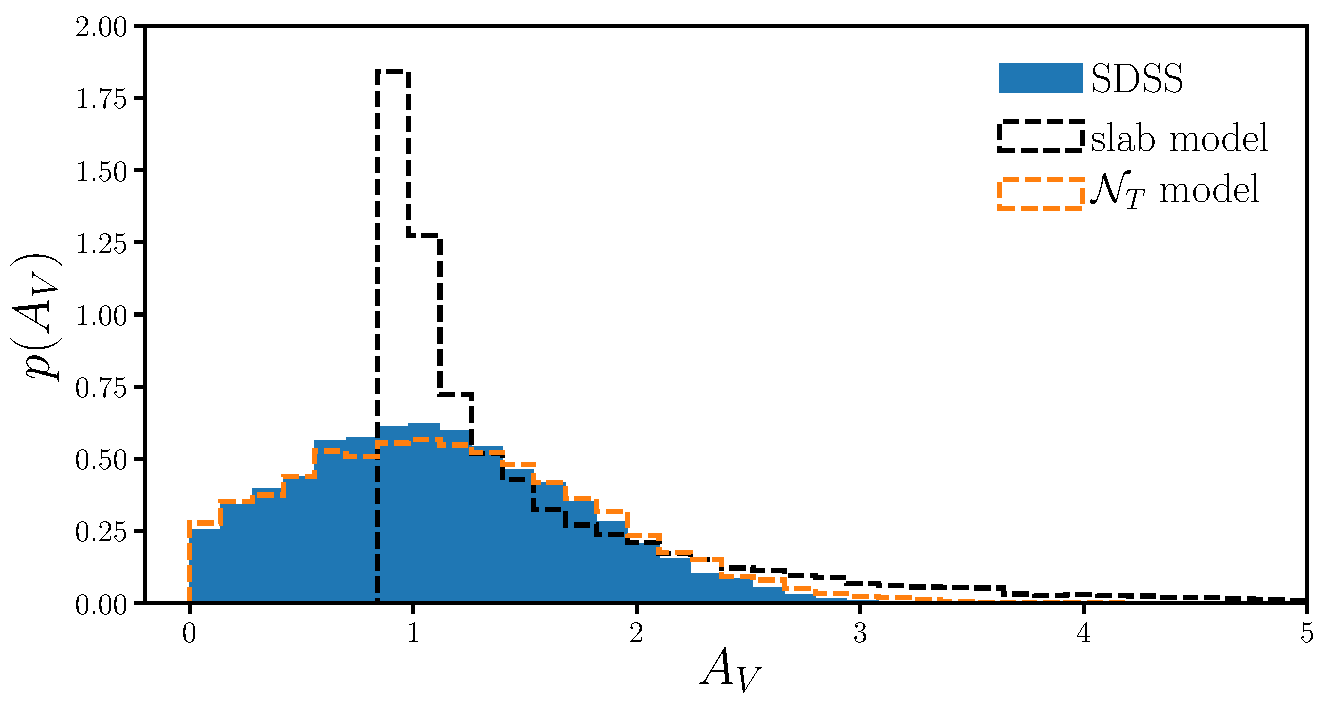
\includegraphics[width=0.66\textwidth]{figs/slab_tnorm.pdf} 
        \caption{\label{fig:av_dist}
            Comparison of $A_V$ distribution of SDSS star-forming
        galaxies (blue) to predictions from the slab model (Eq.~\ref{eq:slab};
        black). {\color{red} detail on how SDSS SF galaxies are classified.} 
        The slab model assumes that there's a slab of dust in front of a galaxy.
        We use $\tau_V=2$ for the slab model above. Regardless of $\tau_V$,
        however, the slab model predicts a significantly more asymmetric and peaked $A_V$ distribution
        than observations. Given this disagreement, {\em we include in our
        analysis a DEM with an empirical prescription for $A_V$ based on a truncated normal 
        distribution, which better reproduce the observed $A_V$ distribution} (Section~\ref{sec:nonslab}). }
    \end{center}
\end{figure}


% In this regard, the slab model is consistent with the correlation between $A_V$ and $i$ found in the literature: edge-on galaxies have higher $A_V$ than face-on galaxies~\citep[\eg][]{conroy2010, wild2011, battisti2017, salim2020}. More
